%
% Fighting Game Notation for LaTeX
%
% MIT License
%
% Copyright (c) 2021 Ian Malerich
%
% Permission is hereby granted, free of charge, to any person obtaining a copy
% of this software and associated documentation files (the "Software"), to deal
% in the Software without restriction, including without limitation the rights
% to use, copy, modify, merge, publish, distribute, sublicense, and/or sell
% copies of the Software, and to permit persons to whom the Software is
% furnished to do so, subject to the following conditions:

% The above copyright notice and this permission notice shall be included in all
% copies or substantial portions of the Software.

% THE SOFTWARE IS PROVIDED "AS IS", WITHOUT WARRANTY OF ANY KIND, EXPRESS OR
% IMPLIED, INCLUDING BUT NOT LIMITED TO THE WARRANTIES OF MERCHANTABILITY,
% FITNESS FOR A PARTICULAR PURPOSE AND NONINFRINGEMENT. IN NO EVENT SHALL THE
% AUTHORS OR COPYRIGHT HOLDERS BE LIABLE FOR ANY CLAIM, DAMAGES OR OTHER
% LIABILITY, WHETHER IN AN ACTION OF CONTRACT, TORT OR OTHERWISE, ARISING FROM,
% OUT OF OR IN CONNECTION WITH THE SOFTWARE OR THE USE OR OTHER DEALINGS IN THE
% SOFTWARE.
%

\documentclass[a4paper,8pt]{letter}
\usepackage[table]{xcolor}
\usepackage{combo,soul,geometry,extsizes,multicol,enumitem,inputenc}
\usepackage[export]{adjustbox}
\usepackage{geometry,tabularx}
\usepackage{anyfontsize,booktabs}

\geometry{
	a4paper,
	total={170mm,257mm},
	left=20mm,
	top=20mm,
}

\pagenumbering{gobble} % disable page numbers
\def\arraystretch{2.0} % increase the height of tabular rows

\begin{document}
\begin{center}
  \makebox[\textwidth]{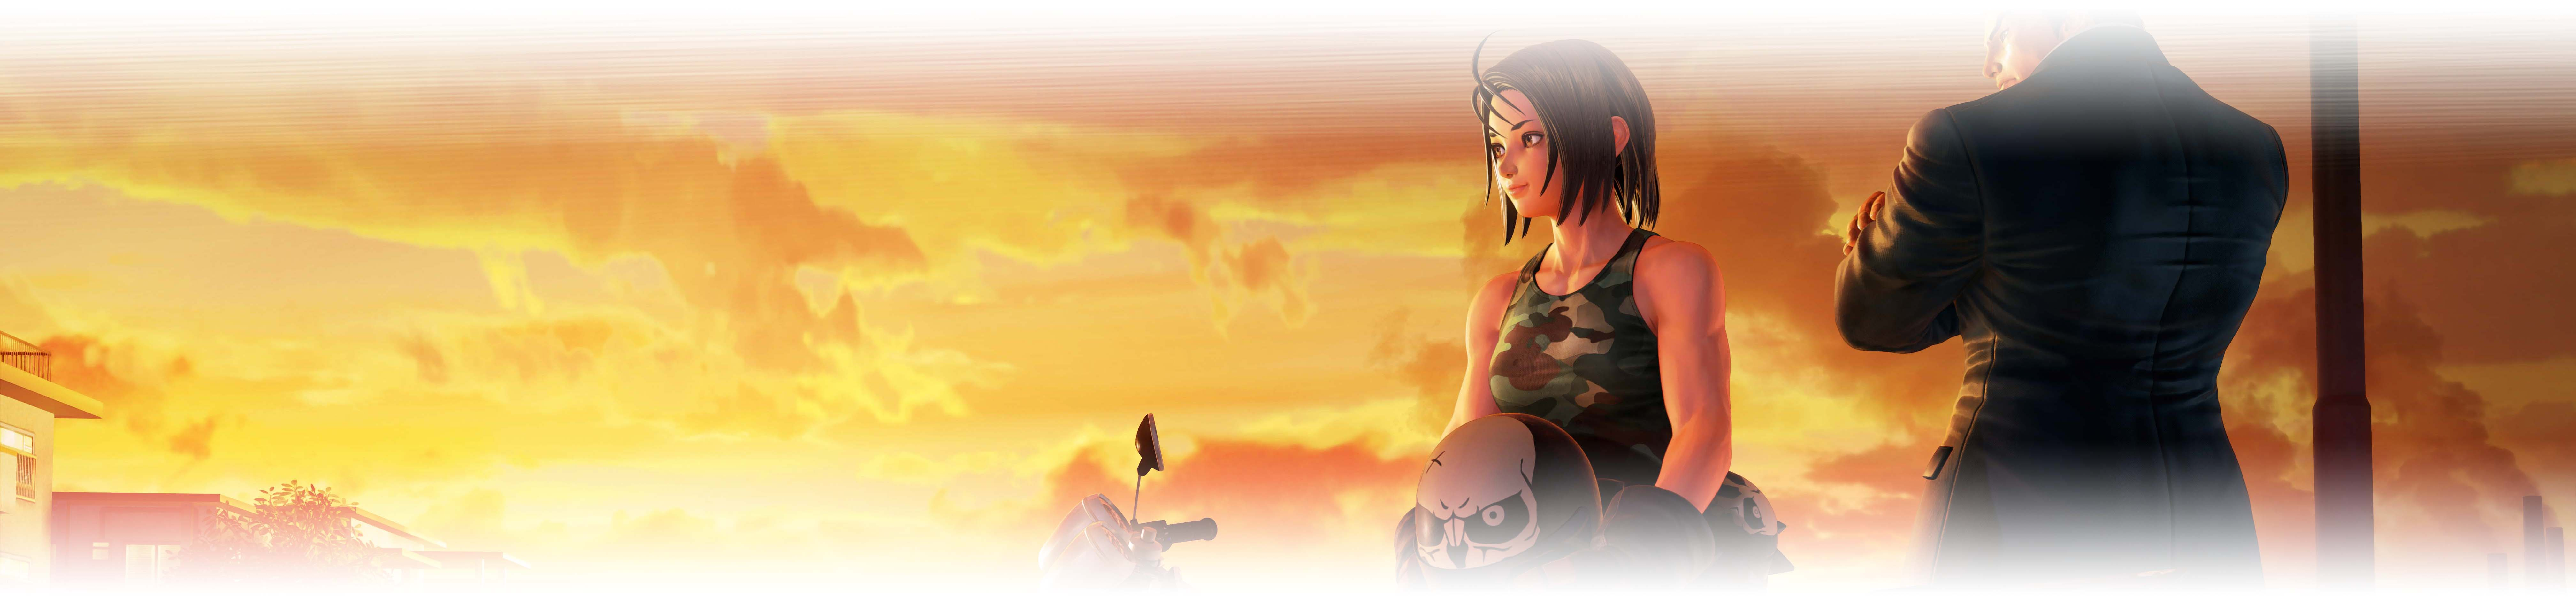
\includegraphics[width=\paperwidth]{akira-A}}
\end{center}
\sffamily
\vspace*{-26ex}
{\fontsize{50}{60} \textbf{\textcolor{black}{Akira}}}
\noindent
\begin{multicols}{2}
\noindent
\rowcolors{2}{gray!20}{white}\begin{tabular}{|p{0.95\linewidth}|}\hline\rowcolor{black!78}
\textcolor{white}{{\small lights}} \\
cr.\lkick, cr.\lpunch\cancel \qcb\lpunch \\
cr.\lkick, cr.\lpunch\cancel \qcb\expunch \\
cr.\lkick, cr.\lpunch\cancel \dragonpunch\hkick \\
(st) cr.\lkick, cr.\lpunch\cancel \qcb\hkick, \hkick \\
cr.\lpunch, \lpunch\~\mpunch\cancel \dragonpunch\hkick \\
cr.\lpunch, \lpunch\~\mpunch\cancel \qcb\mkick, \anykick \\
cr.\lpunch, \lpunch\~\mpunch\cancel \qcb\exkick, \dragonpunch\hkick \\
cr.\lpunch, \lpunch\~\mpunch\cancel \qcb\hpunch \\
cr.\lpunch, \lpunch\~\mpunch\~\vstwo \\
\lpunch, \lpunch\~\mpunch\cancel \dragonpunch\hkick \\
\lpunch, \lpunch\~\mpunch\cancel \qcb\hkick, \hkick \\
\lpunch, \lpunch\~\mpunch\cancel \qcb\exkick, \dragonpunch\hkick \\
cr.\lpunch, \lpunch\~\mpunch\~\vstwo\cancel\up, j.\lpunch, j.\mpunch, j.\hpunch, jf.\hpunch\ \\
cr.\lpunch, \lpunch\~\mpunch\~\vstwo\cancel\up, j.\lpunch, j.\mpunch, j.\hpunch, jf.\hpunch\cancel \qcf\expunch \\
cr.\lpunch, \lpunch\~\mpunch\cancel\qcb\hkick, \hkick, \qcb\lpunch\cancel \qcf\qcf\anypunch \\
(cr) cr.\lpunch, \lpunch\~\mpunch\cancel \qcb\mpunch, cr.\lpunch\cancel \dragonpunch\hkick \\
(st) cr.\lpunch, \lpunch\~ \mpunch\cancel \qcb\hkick, \hkick, \qcb\expunch\ (corner)\dragonpunch\exkick \\
(corner) cr.\lpunch, \mpunch\cancel \qcb\exkick, \qcb\lpunch, \dragonpunch\exkick \\
\vsone, cr.\lpunch, \lpunch\~\mkick\cancel\qcb\hkick, \hkick, \qcf\expunch, \qcf\hpunch \\
\vsone, cr.\lpunch, \lpunch\~\mpunch\cancel \qcf\expunch, \dragonpunch\hkick \\
\vsone, \air\qcf\expunch, \hpunch\cancel \qcb\mpunch, cr.\lpunch\cancel \dragonpunch\hkick \\
\vsone, \air\qcf\expunch\ (far), \qcb\hpunch \\ 
\hline\end{tabular}

\columnbreak
\noindent
\rowcolors{2}{gray!20}{white}\begin{tabular}{|p{\linewidth}|}\hline\rowcolor{black!78}
\textcolor{white}{{\small mediums}} \\
cr.\mpunch, \mpunch\ may be used instead of cr.\lpunch, \lpunch\~\mpunch \\
cr.\mkick\cancel \qcf\lpunch, \lkick\cancel \dragonpunch\hkick \\
cr.\mkick\cancel \qcb\lkick, \lkick or \mkick \\
cr.\mkick\cancel \qcb\exkick, \dragonpunch\hkick \\
cr.\mkick\cancel \dragonpunch\hkick \\
(cr.) cr.\mkick\cancel \qcb\mpunch, cr.\lpunch\cancel \dragonpunch\hkick \\
\mpunch, st./cr.\lpunch\cancel \dragonpunch\hkick \\
\mkick, cr.\lpunch\cancel \dragonpunch\hkick \\
cr.\mpunch, \mpunch\cancel \qcb\hpunch\cancel \qcf\qcf\anypunch \\
\hline\end{tabular}

\noindent
\rowcolors{2}{gray!20}{white}\begin{tabular}{|p{\linewidth}|}\hline\rowcolor{black!78}
\textcolor{white}{{\small heavies}} \\
\hpunch, f.\hpunch, f.\hpunch\cancel \vsone \\
\hpunch\~\ f.\hpunch\cancel\vstwo,\up, j.\mpunch, j.\hpunch, j.\hkick\cancel \qcf\expunch \\
f.\hpunch\ \crush, cr.\mpunch\cancel \qcb\mpunch, cr.\lpunch\cancel\dragonpunch\hkick \\
f.\hpunch\ \crush\cancel \vstwo, \up, j.\mpunch, j.\hpunch, j.\hkick\cancel \qcf\anypunch \\
\vsone\hpunch\cancel \qcf\hpunch, \hpunch\cancel \qcb\hkick, \hkick, \qcb\expunch \\
(cr) \vsone\hpunch\cancel \qcf\hpunch, \hpunch\cancel \qcb\mpunch, cr.\lpunch\cancel \dragonpunch\hkick \\
\vsone \air \qcf\anypunch\ leads to a \crush\ state \\
\hline\end{tabular}

\noindent
\rowcolors{2}{gray!20}{white}\begin{tabular}{|p{\linewidth}|}\hline\rowcolor{black!78}
\textcolor{white}{{\small air-to-air}} \\
j.\mpunch\cancel \qcf\hpunch \\
j.\mpunch, \dragonpunch\hkick \\
j.\mpunch, \qcb\hkick, \hkick, \qcb\expunch \\
\hline\end{tabular}
\end{multicols}

\smallbreak\noindent
\rowcolors{2}{gray!20}{white}\begin{tabular}{|p{\linewidth}|}\hline\rowcolor{black!78}
\textcolor{white}{{\small v-trigger 1}} \\
\hpunch\~\ f.\hpunch\cancel \vtone, cr.\hpunch\back\back, j.\hkick, \qcb\hkick, \hkick, \qcb\expunch, \dragonpunch\exkick \\
\hpunch\cancel \vtone, cr.\hpunch\cancel \vstwo, \qcf\lpunch, j.\hpunch\cancel \qcf\lpunch, j.\hpunch\cancel \qcf\lpunch, j.\hpunch\cancel \qcf\expunch \\
\hline\end{tabular}

\smallbreak\noindent
\rowcolors{2}{gray!20}{white}\begin{tabular}{|p{\linewidth}|}\hline\rowcolor{black!78}
\textcolor{white}{{\small v-trigger 2}} \\
\hkick\cancel\vttwo\cancel \anykick, \anypunch, \anykick, \qcb\expunch \\
f.\hpunch\cancel \vttwo, \hpunch\~\ f.\hpunch\cancel \vttwo \anykick, \anypunch, \anykick, \vsone \qcf\expunch, \dragonpunch\exkick \\
\vsone, j.\hkick, cr.\mpunch, \mpunch\cancel \qcb\hkick, \hkick, \qcf\expunch, \vttwo B+K \\
\vsone, f.\hpunch\cancel \vttwo, \down, \hpunch\~\ f.\hpunch\cancel \vttwo, \down, \mpunch\cancel \qcf\mpunch, \mpunch\cancel \vttwo, \anypunch, \anypunch, \anypunch\cancel \qcf\qcf\anypunch \\
\hline\end{tabular}

\end{document}
